% ------------------------------------------------------------------------ %
% !TEX encoding = UTF-8 Unicode
% !TEX TS-program = pdflatex
% !TEX root = ../Tesi.tex
% !TEX spellcheck = it-IT
% ------------------------------------------------------------------------ %
%
% ------------------------------------------------------------------------ %
% 	NOME CAPITOLO
% ------------------------------------------------------------------------ %
%
\chapter{Configurazione dell'ambiente di sviluppo} % (fold)
%
\label{cap:configurazione}
%
\section{Introduzione}
Prima di procedere cn l'implementazione si è dovuti procedere a configurare l'intero ambiente di sviluppo locale relativo ai framework descritti nel capitolo precedente e al nodo locale della blockchain Quorum. Per lo sviluppo si è scelto di utilizzare un ambiente linux, precisamente Ubuntu 16.04 LTS. \\
La versione della blockchain Quorum utilizzata durante lo sviluppo di questa applicazione è stata la 1.5\footnote{Nel mese di ottobre Quorum è stata aggiornata ad una major version 1.8 per riallinearsi alla blockchain Ethereum (aggiornamento client geth in uso alla versione 1.7) e migliorare la propria gestione dei permessi e della privacy}, caratterizzata da una procedura di configurazione divisa in più step che permette di avere un ambiente Quorum completamente funzionale composto da sette nodi indipendenti. Gli sviluppatori di Quorum consigliano, per questa versione, di utilizzare \emph{Vagrant} e l'hypervisor di \emph{Virtualbox}.%
\section{Vagrant} 
Vagrant è un software open-source progettato per cotruire e mantenere ambienti di sviluppo software portabili, capace di utilizzare i maggiori hypervisor attualmente utilizzati come VirtualBox (scelta predefinita all'atto dell'installazione), Hyper-V, Docker, VMware e KVM. L'idea alla base di questo software risiede nel fatto che mantenere l'ambiente di configurazione diventa particolarmente difficoltoso con l'aumentare delle tecnologie utilizzate in uno specifico progetto. Vagrant semplifica i passi della gestione delle configurazioni software al fine di aumentare la produttività dello sviluppo. Vagrant è scritto in Ruby ma il suo ecosistema supporta quasi tutti i maggiori linguaggi. Il software si basa sul concetto di "box". Una box può essere paragonata ad una scatola contenente il sistema operativo, e tutto quello di cui abbiamo bisogno come i software di base ed ogni loro configurazione associata. Invece le impostazioni del software che regolano la creazione di una determinata box sono racchiuse in un file scritto in ruby denominato \enquote*{VagrantFile}. \\
Quindi, una volta scaricato ed installato sia VirtualBox che Vagrant, il passo successivo è stato quello di customizzare i file di configurazione di Vagrant utilizzati nello sviluppo. Per completezza, i file sono stati inseriti nell' \autoref{cap:codici} relativa ai codici utilizzati nel progetto, nella sezione ~\nameref{cap:vagrantConfig}, contiene:
\begin{enumerate}
	\item la box utilizzata. Nel nostro caso \emph{Ubuntu 16.04.3 LTS} (xenial);
	\item la direttiva che specifica l'esecuzione di un file script di configurazione immediatamente dopo la creazione della box (bootstrap.sh);
	\item il mapping delle porte TCP/UDP tra la macchina guest e la macchina host;
	\item la quantità di memoria allocata alla box.
\end{enumerate}
Il file realizzato per configurare la macchina dopo la sua creazione è denominato \emph{bootstrap.sh} e contiene tutte le direttive per installare tutte le dipendenze di Quorum per avere una blockchain completamente funzionante. La sua esecuzione avrà come risultato:
\begin{enumerate}
	\item l'aggiunta del repository ppa:ethereum/ethereum per avere l'accesso in download dei pacchetti Ethereum necessari in Quorum;
	\item l'installazione di Constellation ed Enclave;
	\item l'installazione di Golang, linguaggio di programmazione denominato "GO" scritto da Google. Il core di Quorum infatti è scritto in GO;
	\item la build dei file sorgenti di Quorum scaricati dal repository di Quorum;
\end{enumerate}
Il risultato di bootstrap.sh è un ambiente Quorum pronto per essere utilizzato. Una volta preparati i file, la procedura automatizzata di installazione e configurazione viene lanciata tramite il comando da shell: \emph{vagrant up}. Terminata la configurazione, è possibile accedere alla macchina (e quindi alla blockchain) tramite il comando da shell: \emph{vagrant ssh} che avrà il seguente output:
%
\begin{figure}[H]
	%
	\centering
	%
	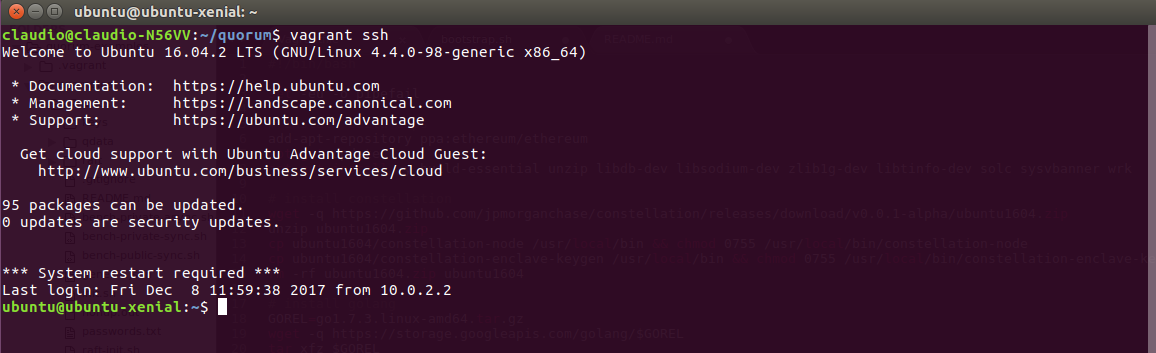
\includegraphics[width=.8\textwidth]{Implementazione/vagrantssh}
	%
	\caption{Terminale per interagire con la blockchain via ssh}
	%
	\label{fig:terminale per interagire con la blockchain}
	%
\end{figure}
%
\section{Quorum}
%
Una volta stabilita la connessione con la macchina virtuale contenente la blockchain, possiamo vedere come l'esecuzione del file bootstrap.sh descritto in precedenza, ha creato due cartelle nella home della macchina:
\begin{itemize}
	\item una cartella \emph{quorum} contenente tutti i file necessari al corretto funzionamento della blockchain;
	\item una cartella \emph{quorum-examples} contenente i file per gestire e personalizzare una istanza locale di Quorum composta da sette nodi indipendenti.
\end{itemize}
Nella cartella \enquote*{quorum-examples/7nodes} troviamo i file per interagire con la blockchain, come possiamo vedere nella seguente immagine:
%
\begin{figure}[H]
	%
	\centering
	%
	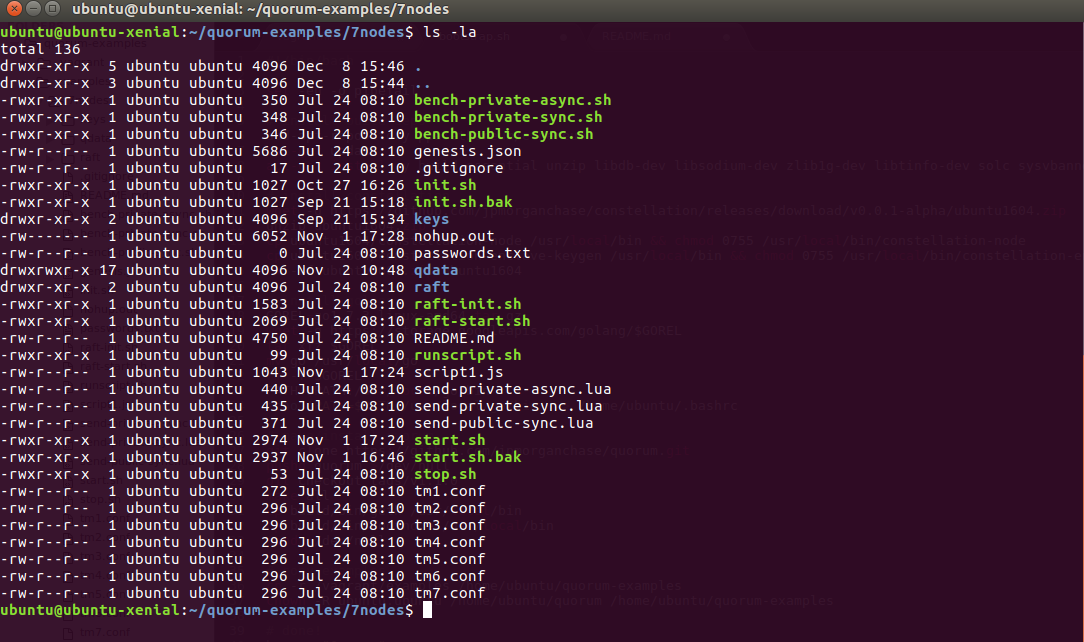
\includegraphics[width=.9\textwidth]{Implementazione/7nodes}
	%
	\caption{Struttura dei file della Blockchain Quorum}
	%
	\label{fig:file blockchain quorum}
	%
\end{figure}
%
In particolare, i file che ci interessano in questa fase di avvio sono:
\begin{enumerate}
	\item \emph{init.sh}. Script da terminale per inizializzare la blockchain. Pulisce le cartelle con i file temporanei locali della blockchain ed inizializza i 7 nodi della blockchain;
	\item \emph{start.sh}. Avvia la blockchain (può accettare ulteriori parametri di configurazione a livello di singolo nodo;
	\item \emph{stop.sh}. Termina tutti i processi della blockchain in modo sicuro.
\end{enumerate}
Questi file, in particolare init.sh e start.sh sono stati modificati per venire incontro alle esigenze dell'applicazione. Anche in questo caso, per l'intera struttura dei file, si rimanda all'\autoref{cap:codici} nella sezione ~\nameref{cap:quorumCode}.
\subsubsection{init.sh}
Il file init.sh è stato riorganizzato al fine di avere, all'avvio della blockchain, due account correttamente configurati sul nodo 1 (dove sarà deployato successivamente il contratto). Per configurare correttamente gli account è necessario:
\begin{enumerate}
	\item per ogni nodo corrispondente viene creata una cartella che andrà a contenere i \emph{keystore} associati ad ogni account e si copiano le informazioni relative alle chiavi pubbliche degli account in ognuna delle cartelle, ove necessario;
	\item si inizializzano i client geth (uno per nodo) tramite i file copiati, a seconda di come si vuole avviare la blockchain, e tramite l'utilizzo ulteriore del file \emph{genesis.json}.
\end{enumerate}
Nel caso invece si vogliano aggiungere ulteriori account, basterà generare tutte le informazioni e le chiavi per il nuovo account tramite Constellation e poi modificare il file init.sh (e lo start.sh di conseguenza).
\subsubsection{start.sh}
Il file start.sh contiente invece i comandi principali per lanciare correttamente l'esecuzione della blockchain. La sua esecuzione ha i seguenti risultati:
\begin{enumerate}
	\item la configurazione del bootnode della blockchain con le direttive a tutte le componenti (eth, web3, quorum ecc);
	\item l'avvio di un'instanza di Constellation per nodo;
	\item l'avvio del bootnode;
	\item l'avvio dei 7 nodi della blockchain. Per lo sviluppo è stata usata la seguente struttura di nodi:
	      \begin{itemize}
	      	\item sul nodo 1 vengono configurati due account, uno dei quali con ruolo voter;
	      	\item sul nodo 2 vengono configurati due account, uno con ruolo voter ed uno con voto maker;
	      	\item nodo 3 configurato senza account;
	      	\item sul nodo 4 viene configurato un nodo voter;
	      	\item i nodi 5,6 e 7 vengono configurati senza account.
	      \end{itemize}
\end{enumerate}
A questo punto la blockchain risulta correttamente configurata ed avviata. Gli account saranno poi associati agli attori dell'applicazione, come vedremo in seguito.
%
\section{Node, Truffle \& Express}
Una volta configurata la blockchain è necessario configurare l'ambiente Node. Per farlo, si devono eseguire i seguenti comandi: 
\begin{itemize}
	\item \textit{\textbf{sudo apt-get install nodejs}}: verrà installata sulla macchina locale l'ultima versione di Node.js\footnote{La versione utilizzata nello sviluppo è stata la v.6.11.1};
	\item \textit{\textbf{sudo apt-get install npm}}: verrà installato il package manager di Node.js.
\end{itemize}
A questo punto è possibile creare la cartella di progetto da dentro cui si andranno ad eseguire i seguenti comandi da terminale:
\begin{itemize}
	\item \textit{\textbf{npm init}}. Questo comando andrà a creare il file \emph{package.json} per l'applicazione, un descrittore json con le informazioni base del progetto e delle sue dipendenze. I campi inseriti sono:
	      \begin{itemize}
	      	\item \emph{name}: nome dell'applicazione;
	      	\item \emph{version}: versione dell'applicazione che, insieme al name, crea un identificatore univoco.
	      	\item \emph{description}: descrizione dell'applicazione
	      	\item \emph{scripts}: dizionario chiave-valore che elenca gli script da lanciare (valore) associati agli eventi del ciclo di vita del progetto (chiave);
	      	\item \emph{dependencies}: contiene le dipendenze necessarie a runtime. Nel nostro caso contiene tutte le librerie per utilizzare correttamente le funzionalità offerte dall'applicazione.
	      \end{itemize}
	\item \textit{\textbf{npm install -g truffle}}: installa globalmente la libreria Truffle;
	\item \textit{\textbf{npm install -g express}}: installa globalmente la libreria Express.
\end{itemize}
A questo punto l'utente ha configurato tutto il necessario e può eseguire il comando \textit{\textbf{truffle init}} che andrà ad inizializzare la cartella di progetto con lo scheletro di progetto di Truffle visto precedentemente. A questo punto, l'ultimo cambiamento da effettuare è la modifica del file truffle.js per farlo puntare verso la blockchain (nel nostro caso è stato scelto il nodo 1 precedentemente configurato), che sarà quindi il localhost sulla porta 22000 (già autorizzata a livello di permessi).
%
\section{Deploy di un contratto sulla blockchain}
%
Una volta configurato truffle per inviare i contratti sulla blockchain si dovrà effettuare quella che viene definita \emph{migrazione}. La migrazione viene realizzata tramite file JavaScript che automatizzano l'attività di deploy del contratto sul nodo di Quorum. Questi file sono scritti in modo tale da poter essere facilmente mantenuti e modificati a seconda di come cambiano le necessità del progetto rispetto al deploy su una particolare blockchain. Si possono avere più file di migrazione all'interno del progetto. \\
Il comando per eseguire la migrazione è \emph{truffle migrate}. Questo comando eseguirà tutti i file di migrazione inseriti nella cartella \emph{migrations/}. Nel caso in cui tutte le migrazioni sono state eseguite con successo, l'esecuzione di truffle migrate partirà dall'ultimo file eseguito, andando ad eseguire solo le nuove migrazioni create. La migrazione verrà eseguita verso il nodo della blockchain specificato nel file \emph{truffle.js}. Per usufruire delle features delle migrazioni di Truffle è necessario avere all'interno del progetto il contratto di migrazione\footnote{Viene configurato in maniera autonoma dal comando \emph{truffle init}} e deve essere deployato come primo contratto nell'ordine di migrazione. \\
Il file di migrazione verso la blockchain Quoruma utilizzato nell'applicazione è il seguente:
\newline	
\begin{lstlisting}[language=javascript,caption={Script di migrazione del contratto dell'applicazione},captionpos=b,frame=lines,basicstyle=\linespread{0.9}\small]
var Prescriptions = artifacts.require("./Prescriptions.sol");
module.exports = function(deployer) {
  deployer.deploy(Prescriptions, {privateFor: ["ROAZBWtSacxXQrOe3FGAqJDyJjFePR5ce4TSIzmJ0Bc="]});
};
\end{lstlisting}
Possiamo vedere la presenza del parametro aggiuntivo, trattato nei capitoli precedenti, denominato \emph{privateFor}. Questo parametro, specifico di Quorum, va ad indicare che il contratto è privato per tutti gli account specificati nell'array privateFor. Questo array andrà a contenere le chiavi pubbliche degli account della blockchain. A questo punto, potranno interagire con il contratto privato tutti gli account la cui chiave pubblica è stata specificata all'atto del deploy e, inoltre, gli account che vorranno effettuare transazioni private dovranno specificare le chiavi pubbliche degli account con cui si vuole interagire all'atto dell'invio della transazione.\\
Lo script completo per il deploy e l'esecuzione dell'applicazione è il seguente:
\newline
\begin{center}
	\begin{lstlisting}[language=sh,caption={Comandi per l'avvio dell'intero ambiente di sviluppo},captionpos=b,frame=lines,basicstyle=\linespread{0.9}\small]
truffle compile && truffle migrate --network quorum && NODE_ENV=development node server.js
	\end{lstlisting}
\end{center}
Questo comando è composto da tre direttive:
\begin{itemize}
	\item \emph{truffle compile}: vengono compilati tutti i contratti presenti nella cartella \emph{contracts/} o, eventualmente, solamente quelli modificati dopo l'ultima compilazione.
	\item \emph{truffle migrate --network quorum}: vengono effettuate tutte le migrazioni dei contratti verso la blockchain in uso.
	\item \emph{NODE\textunderscore ENV=development node server.js}: server.js è il file principale per avviare l'istanza del web server Express (rappresenta il suo entry point)
\end{itemize}
